\def\ktitle{ARM ASSIGNMENT}
\def\kauthor{Marri Srinath Reddy}
\def\kcontact{srinathreddymarri@gmail.com}
\def\kmodule{IITH - Future Wireless Communication}
\documentclass[journal,12pt,twocolumn]{IEEEtran}
\usepackage{enumitem}
\usepackage{tikz}
\usepackage{circuitikz}
\usepackage{karnaugh-map}
\usepackage{tabularx}
\usepackage{circuitikz}
\usepackage{tikz}
\usepackage{titlesec}
\usepackage{multicol}
\title{\ktitle}
\author{\kauthor\\\kcontact\\\kmodule}
\begin{document}
\maketitle
\tableofcontents
\section{\textbf{Question}}
The output expression for the karnaugh map shown below is\\
\resizebox{0.45\textwidth}{!}{%
 \begin{karnaugh-map}[4][4][1][PQ][RS]
  \maxterms{0,2,8,9,10,11}
  \minterms{1,3,4,5,6,7,12,13,14,15}
 \end{karnaugh-map}%
}
\begin{enumerate}[label=(\Alph*)]
 \item $\bar R Q + S$
 \item $Q\bar R + \bar S$
 \item $QR + S$
 \item $QR + \bar S$  
\end{enumerate}
\section{\textbf{Answer}}
The above question can be solved by grouping 1's .Therefore the answer is $\bar R Q + S$\\
\resizebox{0.45\textwidth}{!}{%
 \begin{karnaugh-map}[4][4][1][PQ][RS]
  \maxterms{0,2,8,9,10,11}
  \minterms{1,3,4,5,6,7,12,13,14,15}
            \implicant{4}{14}
             \implicant{1}{7}
 \end{karnaugh-map}%
}
\section{\textbf{Truth Table}}
\begin{tabularx}{0.45\textwidth}{
 | >{\centering\arraybackslash}X
 | >{\centering\arraybackslash}X
 | >{\centering\arraybackslash}X
 | >{\centering\arraybackslash}X
 | >{\centering\arraybackslash}X|
 }\hline
 \textbf{R}&\textbf{S}&\textbf{P}&\textbf{Q}&\textbf{K}\\
 \hline
 0&0&0&0&0\\
 \hline
 0&0&0&1&1\\
 \hline
 0&0&1&0&0\\
 \hline
 0&0&1&1&1\\
 \hline
 0&1&0&0&1\\
 \hline
 0&1&0&1&1\\
 \hline
 0&1&1&0&1\\
 \hline
 0&1&1&1&1\\
 \hline
 1&0&0&0&0\\
 \hline
 1&0&0&1&0\\
 \hline
 1&0&1&0&0\\
 \hline
 1&0&1&1&0\\
 \hline
 1&1&0&0&1\\
 \hline
 1&1&0&1&1\\
 \hline
 1&1&1&0&1\\
 \hline
 1&1&1&1&1\\
 \hline
\end{tabularx}
\begin{center} 
 Truth table for Boolean funtion $K$
\end{center}
\section{\textbf{Logic Diagram}}
\resizebox{0.45\textwidth}{!}{
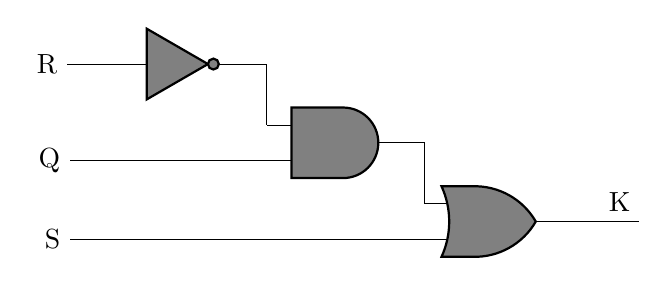
\begin{tikzpicture}
 \ctikzset{
  logic ports=ieee,
  logic ports/scale=0.8,
  logic ports/fill=gray}
 \node[not port](r) at (1,0){};
 \node[and port](a) at (3,-1){};
 \node[or port](b) at (5,-2){};
 \draw(r.out)-|(a.in 1);
 \draw(a.out)-|(b.in 1);
 \draw(r.in 1)-- ++(-0.7,0) node[left]{R};
 \draw(a.in 2)-- ++(-2.5,0) node[left]{Q};
 \draw(b.in 2)-- ++(-4.5,0) node[left]{S};
 \draw(b.out)-- ++(1,0) node[near end,above]{K};
\end{tikzpicture}
}
\begin{center}
 Fig. 2
\end{center}
 \section{\textbf{Components}}
 \begin{tabularx}{0.45\textwidth}{
   | >{\centering\arraybackslash}X
   | >{\centering\arraybackslash}X
   | >{\centering\arraybackslash}X |
   }
   \hline
\textbf{Components}&\textbf{Values}&\textbf{Quantity}\\
   \hline
   VAMAN & & 1\\
   \hline
   Jumper Wires & M-F & 7\\
   \hline
   Breadboard & & 1\\
   \hline
               LED&&1\\
               \hline
               Resistor&100ohms&1\\
               \hline
 \end{tabularx}
\section{\textbf{Implementation}}
\begin{tabularx}{0.45\textwidth}{
  | >{\centering\arraybackslash}X
  | >{\centering\arraybackslash}X
  | >{\centering\arraybackslash}X|}
\hline
 \textbf{VAMAN PIN}&\textbf{INPUT}&\textbf{OUTPUT}\\
 \hline
 23&R& \\
 \hline
 24&S&\\
 \hline
 25&P&\\
 \hline
 22&Q&\\
 \hline
 21&&K\\
 \hline
\end{tabularx}\\
\\
\centering
Connections\\
\textbf{Procedure}
\begin{enumerate}[label={\arabic*}.]
 \item Connect the circuit as per the above table.
 \item Connect inputs to Vcc for Logic 1, ground for Logic 0.
 \item Execute the circuit using the below codes.\\
  \vspace{\baselineskip}
                \begin{tabularx}{0.45\textwidth}{
    | >{\centering\arraybackslash}X|}
   \hline
			https://github.com/SrinathReddyMarri/FWC/\\
			blob/master/ARM/main.c\\
   \hline
  \end{tabularx}
  \vspace{\baselineskip}\\
 \item Change the values of $R,S,P,Q$ in the Hardware and verify the Truth Table.
\end{enumerate}
\end{document}
